\documentclass[11pt]{article}

\usepackage{graphicx}
\usepackage[colorlinks]{hyperref}
\usepackage[margin=0.7in]{geometry}
\usepackage{authblk} % For author and affiliation blocks
\usepackage{tgpagella}
\usepackage{amsmath}
\usepackage{multicol}
\usepackage{float}



\setlength{\columnsep}{0.7in}
% --------------------------------------------------------
% Title and Author Configuration
% --------------------------------------------------------
\title{\textbf{Introduction to State Space Models (SSM)}}

\author[]{Vinay}
\author[]{Subhadeep Sing}
\author[]{Vaibhav Mahore}
\author[]{Snehal Biswas}


\affil[]{Indian Institute of Science, Bangalore \\
\texttt{\{vinay2023 ,shubadeeps ,mvaibhav ,snehalbiswas\}@iisc.ac.in}}




\date{March 18, 2025} % Customize or remove

% --------------------------------------------------------
% Begin Document
% --------------------------------------------------------
\begin{document}

\maketitle
\begin{center}
    \begin{abstract}
        This is a short abstract summarizing the paper.
    \end{abstract}
\end{center}

% Your introduction goes here.
\section{Introduction}
State Space Models (SSMs) have emerged as a promising alternative  to RNN \& LSTM.
This paper explores the need for SSMs in overcoming the challenges faced by conventional
recurrent models. We begin by examining the limitations of RNNs and LSTMs when 
processing long sequences. Then, we present the mathematical principles explaining
the effectiveness of LSSL and HiPPO, setting the stage for an in-depth discussion of the S4 model and  
MAMBA architecture. MAMBA achieves state-of-the-art performance across several modalities such as language, audio, and 
genomics. On language modeling, Mamba-3B model outperforms Transformers of the same size and matches Transformers 
twice its size, both in pretraining and downstream evaluation. \href{https://arxiv.org/abs/2110.13985.pdf}{[1]}


\section{Related Work}
% Discuss related research, references, etc.

\section{Method}
% Detailed description of your proposed method or replication steps.

\section{Experiments}
% Describe experiments, datasets, metrics, etc.

\section{Conclusion}
% Conclude with key insights and future directions.
\appendix
\section*{Appendix}
\addcontentsline{toc}{section}{Appendix}
\section{RNN}

\subsection{Structure of RNN}

RNNs are designed to process sequential data by maintaining a hidden state that
captures information about previous inputs. The basic architecture consists of an input
layer, a hidden layer, and an output layer. Unlike feedforward neural networks, RNNs
have recurrent connections, as shown in Figure 1, allowing information to cycle within the
networks. At each time step, t, the RNN takes an input vector $x_t$  and updates its hidden state, $h_t$, using the following equation: 

\[
h_t = \sigma_h (W_{xh} x_t + W_{hh} h_{t-1} + b_h),
\]

where \( W_{xh} \) is the weight matrix between the input and hidden layer, \( W_{hh} \) is the weight matrix for the recurrent connection, \( b_h \) is the bias vector, and \( \sigma_h \) is the activation function, typically the hyperbolic tangent function (\(\tanh\)) or the rectified linear unit.
 The output at each time step, \( t \), is given by the following:

\[
y_t = \sigma_y(W_{hy} h_t + b_y),
\]

where \( W_{hy} \) is the weight matrix between the hidden and output layers, \( \mathbf{b}_y \) is the bias vector, and \( \sigma_y \) is the activation function for the output layer.

\begin{figure}[h]
    \centering
    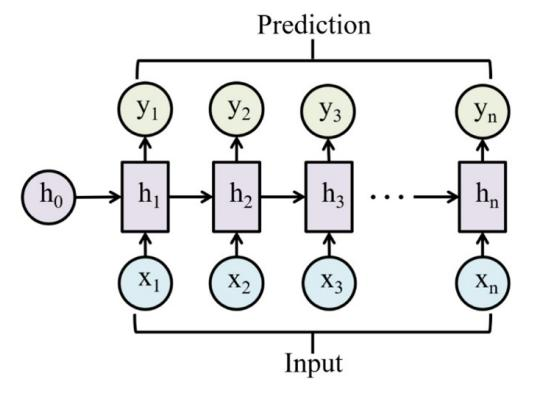
\includegraphics[width=0.32\textwidth]{rnn.png}
    \caption{RNN architecture}
    \label{fig:rnn_structure}
\end{figure}



\subsection{Vanishing and Exploding Gradient}

Training RNNs is challenging due to the vanishing and exploding gradient problems. The BPTT algorithm computes gradients of the loss function, but as they propagate backward, they may vanish or explode, hindering long-term dependency learning or causing instability. The hidden state at time step \( t \) expands as:  

\begin{equation}
h_t = \sigma_h(W_{xh} x_t + W_{hh} \sigma_h(W_{xh} x_{t-1} + W_{hh} h_{t-2} + b_h) + b_h)
\end{equation}

Gradients involve Jacobian matrix products:  

\begin{equation}
\frac{\partial h_t}{\partial h_{t-n}} = \prod_{k=t-n}^{t-1} J_k
\end{equation}

where \( J_k \) is the Jacobian at time \( k \). If its eigenvalues are \( <1 \), gradients vanish, weakening updates for earlier layers. If \( >1 \), gradients explode, causing instability or convergence to poor minima.  

To address this, RNN variants like LSTM use gating mechanisms to regulate information flow and improve long-term dependency learning.
\section{LSTM}
LSTMs overcome these issues by maintaining long-term memory, allowing 
them to use both short-term and long-term memory together. This combination enables more accurate predictions 
for tasks where context over longer sequences is crucial. Now, let us explore the working principles of Long Short-Term Memory (LSTM) networks.

\begin{figure}[H]
    \centering
    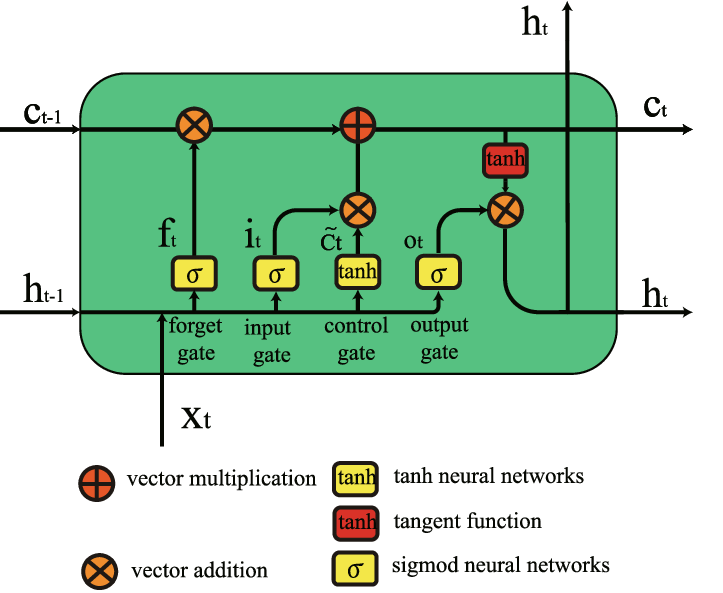
\includegraphics[scale=0.45]{LSTM.png} % Replace with your actual image file name
    \caption{LSTM Architecture}
    \label{fig:myimage}
\end{figure}


{\small
\[
    \begin{aligned}
        f_t &= \sigma\bigl(W_f [h_{t-1}, x_t] + b_f\bigr) &C_t &= f_t \times C_{t-1} + i_t \times \tilde{C}_t,\\
        i_t &= \sigma\bigl(W_i [h_{t-1}, x_t] + b_i\bigr), &o_t &= \sigma\bigl(W_o [h_{t-1}, x_t] + b_o\bigr),\\
        \tilde{C}_t &= \tanh\bigl(W_C [h_{t-1}, x_t] + b_C\bigr), &h_t &= o_t \times \tanh\bigl(C_t\bigr).
    \end{aligned}
\]

}



The core idea behind LSTM is the horizontal line running across the top of the diagram. It extends straight down the entire chain with only minor modifications, allowing information to flow along it unchanged.

The gates are designed to optionally permit information to pass through. They consist of sigmoid layer outputs that produce values between 0 and 1, indicating how much of each component should be allowed to pass.
{\small
\paragraph{Step 1: Forget Gate}
The forget gate decides which information to discard from the cell state. It takes the previous hidden state \(h_{t-1}\) and the current input \(x_t\) as input and outputs values between 0 and 1 for each component in \(C_{t-1}\):  
\[
f_t = \sigma\bigl(W_f [h_{t-1}, x_t] + b_f\bigr).
\]
}
{\small

\paragraph{Step 2: Input and Update}  
This step consists of two parts. First, the input gate, a sigmoid layer, decides which values to update:  
\[
i_t = \sigma\bigl(W_i [h_{t-1}, x_t] + b_i\bigr).
\]  
Next, a tanh layer generates candidate values \(\tilde{C}_t\) for updating the cell state:  
\[
\tilde{C}t = \tanh\bigl(W_C [h{t-1}, x_t] + b_C\bigr).
\]  
The new cell state is then computed by combining the previous state and the new candidate values:  
\[
C_t = f_t \times C_{t-1} + i_t \times \tilde{C}_t.
\]  
}
{\small
\paragraph{Step 3: Output Gate}
For the output, a sigmoid layer determines which parts of the cell state to emit:
\[
o_t = \sigma\bigl(W_o [h_{t-1}, x_t] + b_o\bigr).
\]
Then, the cell state \(C_t\) is passed through a tanh function (to constrain values between \(-1\) and \(1\)) and multiplied by \(o_t\) to obtain the new hidden state:
\[
h_t = o_t \times \tanh\bigl(C_t\bigr).
\]
}

\section*{References}
\bibliographystyle{plain}
\bibliography{references}
[1] . 
[2] . 
[3] . 
[4] . 
[5] . 
[6] . 
[7] . 
[8] . 


\end{document}
